\section{Lösungsstrategie}
Top level architecture
Technologyy decisions
Architectural pattern / Desgin pattern
Development process
Abstract, highest-level architecture or solution concept. Show blocks that address (solve) the prior context diagram. How are you structuring the system to achieve the system goal? Without going into the details that the next section goes into (packages and classes).
Architecture Drivers: : see table example in software architecture course slides
Architecture Principles/Pattern: : see table example in software architecture course slides
Table with Cross-Mapping of Architecture Principles to/from Architecture Drivers: see table example in software architecture course slides

\subsection{Service-Diagramm}

\begin{figure}
    \centering
    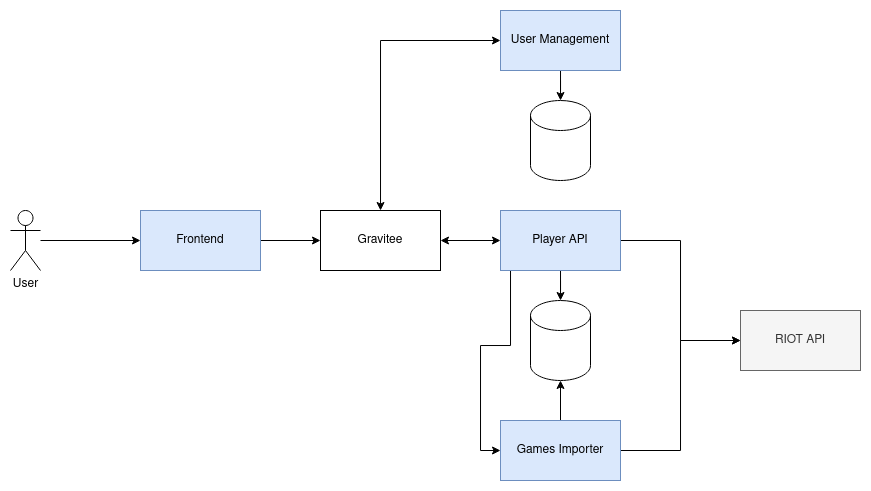
\includegraphics[width=\textwidth]{images/cdc-05-service-diagram.drawio}
    \caption{Service Diagramm der Applikation}
    \label{fig:service-diagram}
\end{figure}

In Abbildung~\ref{fig:service-diagram} ist das Service Diagramm für die Applikation zu sehen.
% TODO: ausformulieren

\subsection{Technolgien}

\subsubsection{Games Importer}\label{subsubsec:games-importer}
Dieser Service ist die Verbindung zwischen der Riot API und unserer Anwendung. Er läuft in seinem eigenen Docker Container. Hier werden die Daten aus der Riot API abgefragt und dann in unserer Datenbank gespeichert.\\
Der Service ist in Python geschrieben, da hierfür bereits Libraries zur Kommunikation mit der Riot API vorhanden sind (siehe \ref{riot-api-libraries}).\\
Neben den Riot API Wrappern Cassiopeia und Riot Watcher wird noch das psycopg2 Package verwendet, welches Zugriff auf die PostgreSQL Datenbank bietet. Psycopg2 erlaubt es in Python SQL Statements zu bauen und auszuführen um somit die Daten von der Riot API in der Datenbank zu speichern.\\
Der Games Importer Service läuft dauerhaft und aktualisiert in 5min Abständen alle in der Datenbank gespeicherten Spieler. \\
Des weitere läuft in deinem weiteren Thread eine GRPC Connection, welche es erlaubt den Import eines neuen Spieler anzufragen. Dieser wird dann erstmals von der Riot API in die Datenbank importiert und bei den zukünftigen Updates berücksichtigt.

\subsubsection{LoL Database}
Die PostgreSQL Datenbank läuft in einem eigenen Docker Container. In dieser Datenbank werden alle Spieler bezogenen Daten gespeichert, welche auf der Website angezeigt werden.\\
Die Daten werden alle vom Games Importer Service aus der Riot API gelesen und in dieser Datenbank gespeichert. Der Player API Service kann dann auf diese Daten zugreifen um sie an das Frontend weiterzugeben.

\subsubsection{Player API}

Dieser Service stellt die importierten Daten des Service~\ref{subsubsec:games-importer} dar.
Als Programmiersprache um eine schnelle Entwicklung zu erreichen und um im Backend nur eine Sprache zu verwenden.
Als Webframework wurde sich für FastAPI entschieden, aufgrund der hohen Performance.
Für den Datenbankzugriff wurde sich für SQLAlchemy entschieden, um ein ORM verwenden zu können.

\subsubsection{User Management}

\subsubsection{Frontend}

Über das Frontend lässt sich die Anwendung benutzen. Sie ist derzeit für die Benutzung mit dem Webbrowser ausgelegt. Dabei kommen folgende Technolgien zum Einsatz.  \\

\textbf{NuxtJS} \\

Für die Umsetzung des reaktiven Frontends wurde das "NuxtJs"-Framework (\href{https://nuxtjs.org/}{https://nuxtjs.org/}) entschieden. Dieses erlaubt es komplexe Vue-Anwendungen umzusetzen und unterstützt Entwickler:innen
bei unterschiedlichen Problemstellungen der Frontend-Entwicklung. Aufgrund bereits existierender Erfahrung mit Vue und dem Framework viel die Wahl auf diese Technologie.
Dadurch ist eine rasche Entwicklung gewährleistet, indem die Einarbeitungszeit in neue Technologien wegfällt. Die Kommunikation mit verschiedenen Diensten passiert
über das HTTP-Protokoll. Mit dem eingebauten Modul "Axios", welches als HTTP-Client dient, werden HTTP-Anfragen an das Backend gesendet, um die entsprechenden Daten 
zu erhalten. Zur Authentifizierung der Benutzer:innen wird das Modul "NuxtJs Auth" (\href{https://auth.nuxtjs.org/}{https://auth.nuxtjs.org/}) verwendet. Dieses stellt eine API zur Verfügung, mit der Registierungs- und Anmeldeprozess durchgeführt werden kann.
Ebenso übernimmt es die Speicherung und Verifizierung des vom User-Backend erhaltene JWT-Token. \\

\textbf{Design} \\

Um ein einfache, responsive und übersichtliche Web-Oberfläche den Nutzer:innen zu gewährleisten, viel die Wahl auf "Tabler" (\href{http://tabler.io/}{http://tabler.io/}). Dies ist ein freies Frontend-CSS-Framework
und stellt das Grundgerüst einer Administrationsoberfläche zur Verfügung. Aufgrund zahlreicher HTML-Module kann die Benutzeroberfläche nach Belieben konzeptioniert und 
umgesetzt werden. Ebenso bietet diese CCS-Framework bereits ein responsives Layout, wodruch zeitgleich die Benutzeroberfläche automatisch für mobile Endgeräte angepasst wird.

\subsection{Architektur}

In den beiden Tabellen~\ref{tab:goals} und~\ref{tab:principles}, werden die Ziele der Architektur aufgelistet
und die jeweiligen Architektur Prinzipien, die diese unterstützen.

\subsubsection{Drivers}
\begin{center}
    \begin{tabular}{|l|l|l| p{5cm} |p{2.5cm}|}
        \hline
        \textbf{Priorität} & \textbf{Arch. Ziel (AG)} & \textbf{Abkürzung} & \textbf{Eigenschaften} & \textbf{Unterstützt von APs?} \\
        \hline
        1 & Funktionalität & AG:FUNC & UI, Business Logik, Daten & AP:SOA \\
        2 & Benutzbarkeit & AG:USA & responsive ui &  \\
        3 & Portabilität & AG:PORT & DB, OS Unabhängigkeit & AP:PY AP:DOCKER AP:ORM\\
        4 & Interoperabilität & AG:INT & RDB Austauschbarkeit & AP:ORM \\
        5 & Wartbarkeit & AG:MTN & & AP:SOA AP:PY AP:DOCKER AP:ORM\\
        6 & Performance & AG:PERF & Latenz & AP:POLL \\
        7 & Ausfallsicherheit & AG:RLB & ACID Transaktionen, unabhängige Services & AP:SOA AP:RDB AP:DOCKER\\
        8 & Security & AG:SEC & Passwörter hashen, Kommunikation über https &  \\
        \hline
    \end{tabular}
    \label{tab:goals}
\end{center}
\subsubsection{Prinzipien}

\begin{center}
    \begin{tabular}{|l|l| p{5cm} |p{3cm}|}
        \hline
        \textbf{Arch. Prinzip (AP)} & \textbf{Abkürzung} & \textbf{Beschreibung.} & \textbf{Unterstützt AGs} \\
        \hline
        Service orientiert & AP:SOA & Backends aufgeteilt auf Services um Requests zu händeln & AG:FUNC AG:MTN AG:RLB \\
        Relationale DB & AP:RDB & Daten in relationaler Datenbank mit SQL gespeichert & AG:RLB \\
        Python & AP:PY & Python ist OS unabhängig und ermöglicht gute Wartbarkeit & AG:PORT AG:MTN \\
        Docker & AP:DOCKER & Docker erlaubt unabhängiges und einfaches deployment & AG:MTN AG:PORT AG:RLB \\
        OR Mapping & AP:ORM & Datenbankunabhängigkeit und einfaches Entwickeln & AG:PORT AG:INT AG:MTN \\
        Polling & AP:POLL & Polling statt lang wartende Requests ermöglicht schnelle Antworten & AG:PERF \\
        \hline
    \end{tabular}
    \label{tab:principles}
\end{center}
